\chapter{Project Development}\label{chap:project}

Considering the classification presented in ``Metabolic Disease", published by ``Encyclopedia Britannica"~\cite{britannica}, the class of metabolic diseases around which the implementation will be oriented is ``disorders of amino acid metabolism". In particular, the diseases selected for the study are twelve: ``Phenylketonuria" (PKU), ``Tyrosinemia Type I", ``Tyrosinemia Type II", ``Tyrosinemia Type III", ``Homocystinuria", ``Hyperglycinemia, ``OTC Deficiency", ``Cystinuria", ``Lisinuric Protein Intolerance" (LPI), ``Propionic Acidemia", ``Methylmalonic Acidemia" and ``Maple Syrup Disease" (MSP).

\section{Pathways Selection}

The first essential step of the project, after an initial theoretical research phase, consisted in selecting, downloading and combining metabolic disease pathways extracted from ``Reactome''~\cite{reactome}. In particular, two types of pathways were selected: those relating to the specific twelve diseases highlighted in the previous section, and those relating to ``healthy" metabolic processes, so as to integrate information on nodes and edges that were absent in diseases' pathways due to the fact that these may inhibit or alter certain processes. All data downloaded from ``Reactome"~\cite{reactome} and generally used in this first phase are collected in the project's ``./data" folder.

\section{Integration of drug interactions}
The reference source for known drugs for each of the diseases investigated, as well as for each of the drugs evaluated in the rankings, is ``DrugBank"~\cite{drugbank}.
A design choice applied at this stage was to consider all and only the drugs belonging to the file ``pharmacologically\_active.csv" found in ``Drugbank"~\cite{drugbank}. This is because, since the implementation approach is based on distances in a graph, this would penalise in the ranking phase all the drugs that by their very nature do not interact directly with the diseases under examination, and would therefore make the system heavier and slower, while not providing important contributions to the results.

This step resulted in the addition to the graph of nodes representing the 2220 drugs under consideration for each disease rankings, including the 14 drugs known for the treatment of the 12 metabolic diseases under consideration.
Each drug node has edges pointing to each of the targets of the specific drug it models, also represented by nodes in the graph. Finally, at the end of this step, as well as at the end of the production of the final complete graph, each node will represent a specific biological entity, unique in the whole graph and source of hedges modelling every useful known interaction of the component, pointing to each of the nodes it interact with.

\section{Graph enrichment and completion}
Exploiting ``BioGRID"~\cite{biogrid}, the aim of this step was to integrate novel information (node and edges - components and interactions) to enrich the already built graph. In particular, the components selected as a starting point for integration where all the genes present in the graph, both from diseases and drugs. The new data where acquired by performing queries on the server, specifying the genes of interest, and using a  file (``BIOGRID-ORGANISM-Homo\_sapiens-4.4.221.tab3.txt"), containing all interactions in the human body, subsequently filtered. 

\section{Ranking algorithm}

As the focus during development was more directed toward the study of data structures and results interpretation, the implementation of the algorithm for the calculation of rankings is based on a simple and basic approach. Nevertheless, however, the project produced interesting results that will be evaluated and validated in the next sections. 

The implemented algorithm calculates, for each drug, the average distance that the node that models it in the graph has with respect to the various components of the disease under examination. This exploiting also the hereditary nature of the metabolic diseases, that permits the approximation on the components (represented by nodes) of those diseases as the genes which are in any sense involved in those diseases' pathways.

%\begin{center}
%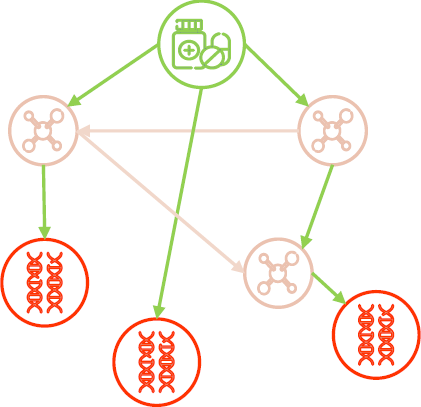
\includegraphics[width=4cm]{Images/interactions.png}
%\end{center}


\section{Validation}
After the ranking phase, a series of four validations were conducted: first a set of two qualitative validations and than another set of two statistical validations:
\begin{itemize}
    \item \textbf{first qualitative test}: the purpose of the test is to verify that known drugs are at the top of the rankings for their respective (target) diseases. 79.17\% of drugs qualify in high rankings for their target diseases;
    \item \textbf{second qualitative test}: the objective of the test is to verify that for each known drug, the mean rank achieved in its target disease ranking is higher than the mean rank achieved by the same drug in non target diseases ranking. A total of 3 out of 14 drugs fail this test; 
    \item \textbf{first statistical test}: the aim of the test is the same as the previous one, but in this case a statistical validation is performed through a t-test.
    The test is performed on two vector: the first containing the rankings of known drugs towards the respective target diseases, while the second contains the rankings of the same drugs but for diseases not yet related to these drugs.
    The p-value obtained for this test is lesser than 0.05, which tests that, for diseases under consideration, known treatment drugs are better classified than unknown ones;
    \item \textbf{second statistical test}: via t-test, this test shows that, considering all the rankings, the 14 known drugs have a better rank than randomly taken drugs.
    The test is performed on two vector: the first is identical to the first of the previous test, while the second one contains the 1680 ranks (14 different randomly extracted drugs in the 12 diseases rankings, repeating the process in 10 times iterations).
    As a result, the p-value computed is lesser than 0.05, which demonstrate that known drugs are ranked better than randomly taken drugs.
\end{itemize}

% rimando al fatto che i risultati sono in un capitolo a parte